% ============================================================
% IE UNIVERSITY - BACHELOR IN APPLIED MATHEMATICS
% MACHINE LEARNING & COMMUNICATION SKILLS PROJECT - PROGRESS REPORT
% Uses the official proposal class with the header changed to "Progress Report".
% Citations follow MLA (author-title in text, Works Cited list), as required by the
% project guidelines.
% ============================================================

\documentclass[clean]{bam-progress}

\BAMtitle{FIELD: How Much Does the Field of Study Shape University GPA Rankings?}
\BAMteam{Adam Bajer; Pablo Torres; Ignacio Gimeno}
\BAMcourse{Machine Learning \& Communication Skills}
\BAMacademicyear{2026--2027}
\BAMsubmissiondate{25 October 2026, 23:59 Madrid time}

\begin{document}
\makeproposalheader

\noindent\textit{FIELD: Field Influence on Evaluation Levels across Degrees.}

% ============================================================
\section{Interpreting the Proposal Result}

In the proposal, the field of study alone predicted how far a field's mean grade sits from its university's average. The feedback asked what that means, and the answer decides where FIELD goes next. If a field sat at the same distance from its university average everywhere, we would be looking at universal field effects; if the distance varied from one university to another, the variation itself would need an explanation. Overall grade levels of universities play no part in our models, because the target is always a field's mean minus the average of all fields in the same university and year.

% ============================================================
\section{Results}

\subsection{Shared and university-specific field effects}

We decomposed 12,125 university-field-year means (89 universities, 29 fields, 2015--16 to 2023--24) from the Ministry of Universities (Ministerio de Ciencia, Innovaci\'on y Universidades, ``Media, cuartiles'') with nested linear models. University-year averages explain 20\% of the variation. Within each university-year, 65\% of what is left is a field effect shared by all universities, 28\% is specific to each university (a statistically significant difference, $p < 0.001$) and the remaining 7\% is year-to-year noise. The university-specific part is stable: a field's deviation in one year is strongly correlated with the same university and field the next year ($r = 0.84$ over 10,413 pairs; Figure~\ref{fig:persistence}).

\subsection{Comparison of models}

We trained each model on 2015--2021 and tested it on 2022--2023, using the 2,774 university-field-years (87 universities) whose university and field appear in the training years (Table~\ref{tab:models}). With the shared field effect the test error falls from 0.365 to 0.226 grade points. Gradient boosting that also uses dropout and size gets to 0.206, and a ridge model with a separate term for each university and field gets to 0.137, with an interval that does not overlap with any other model's. How a university graded its fields before is the best predictor of how it grades them later, which confirms the decomposition on unseen data. In the Portuguese student records (Realinho et al.), adding the degree to a logistic regression for reaching the top 20\% by raw GPA raises the AUC from 0.699 to 0.744, so the degree still predicts who reaches the top of a pooled ranking once entry profiles are taken into account.

\begin{table}[htbp]
  \centering
  \caption{Comparison of models. Spain: RMSE (grade points, 5--10 scale) of a field's deviation from its university-year average in 2022--2023; the intervals come from 1,000 bootstrap resamples of universities. Portugal: AUC for being in the top 20\% by raw GPA, from 10-fold cross-validation; $\pm$ is the standard deviation across folds.}
  \label{tab:models}
  \begin{tabularx}{0.92\linewidth}{@{}Xc@{}}
    \toprule
    Model & Test metric \\
    \midrule
    \multicolumn{2}{@{}l}{\emph{Spain: RMSE (lower is better)}} \\
    Baseline: zero deviation & 0.365 (0.348--0.381) \\
    Ridge: shared field effect & 0.226 (0.211--0.241) \\
    Gradient boosting: field, dropout rate and size & 0.206 (0.193--0.220) \\
    Ridge: shared + university-by-field effect & 0.137 (0.128--0.148) \\
    \midrule
    \multicolumn{2}{@{}l}{\emph{Portugal: AUC (higher is better)}} \\
    Logistic: degree only & $0.656 \pm 0.036$ \\
    Logistic: standardised entry grades and background & $0.699 \pm 0.042$ \\
    Logistic: standardised entry grades, background and degree & $0.744 \pm 0.032$ \\
    \bottomrule
  \end{tabularx}
\end{table}

\subsection{Possible confounders}

We added the admission grade of new entrants, the number of graduates and the dropout rate from further Ministry tables (Ministerio de Ciencia, Innovaci\'on y Universidades, ``Tasas de abandono''; ``Egresados''; ``Nota media \ldots{} rama''; ``Nota media \ldots{} \'ambito''). Raw entry grades are not comparable across groups, so we standardised them: Spanish branch averages (5--14 scale, public universities only) became $z$-scores, and Portuguese grades were standardised within each admission route, because routes grade applicants differently. Fields with higher national admission grades do not have higher field effects (no significant relation). Inside the 47 public universities, fields with stronger intakes have slightly higher grades, yet adding intake and size leaves the field effects almost exactly as they were (Figure~\ref{fig:confounders}). In the Portuguese records the gap between the highest- and lowest-graded degree only shrinks from 1.51 to 1.30 points on the 0--20 scale, and the difference between degrees remains statistically significant. Dropout matters more, cutting the spread of field effects from 0.31 to 0.24 points. We kept it out of the main controls because low grades may be one of the reasons students leave. Grouping the fields with $k$-means and plotting them with PCA points the same way: fields with high dropout and lower grades, such as Engineering and Economics, end up on one side, and fields with low dropout and higher grades, such as Nursing and Medicine, on the other.

\subsection{Selection under different ranking rules}

Weighting the selection simulation by the number of graduates (664 university-years), the median university-year places 41\% of Nursing graduates in its top 20\% (interquartile range 29--54\%), compared with 6\% (2--13\%) in Business Administration. We also tried four ranking rules on the Portuguese data. With raw GPA the share of students selected varies a lot between degrees (a spread of 8.1 percentage points); regression-adjusted GPA reduces it to 3.6, a within-degree $z$-score to 1.9 and within-degree percentiles to 0.4. The selected students' entry grades barely change between rules.

\subsection{What the results rule out and what they leave open}

Two explanations now look unlikely. Overall differences between universities cannot produce our field gaps, since they are removed by construction, and differences in intake explain only a small part of them. What remains are field gaps that are partly shared across Spain and partly specific to each university, and both parts persist over time. The data cannot yet tell us why: a university-specific gap may come from grading practice, from course content, or from abilities that admission grades do not measure. The dropout pattern adds a further caution. Because the data only include graduates, fields that lose more students are compared on a more selected group, so the observed gaps are probably smaller than the real ones.

% ============================================================
\section{Issues, Decisions and Next Steps}

University admission grades exist only for public universities and five broad branches, so private universities are left out of the confounder analysis and fields are mapped to branches approximately. The Ministry hides small cells, leaving about half of the university-field-years empty; the models use only reported cells. Compared with the proposal, we now remove university-by-year effects, standardise entry grades and keep dropout apart from the intake controls. For the Sentence Outline we plan to fit a mixed-effects model with random university-by-field effects, which estimates each university's profile with partial pooling and uncertainty; check the normal approximation used in the simulation; replicate the shared effects on the US dataset of 33 universities (Jeong et al.); and compare the ranking rules against one common criterion. Every result comes from Python scripts with fixed seeds.

% ============================================================
% Figures and references follow the two pages of text.
\clearpage
\begin{figure}[h!]
  \centering
  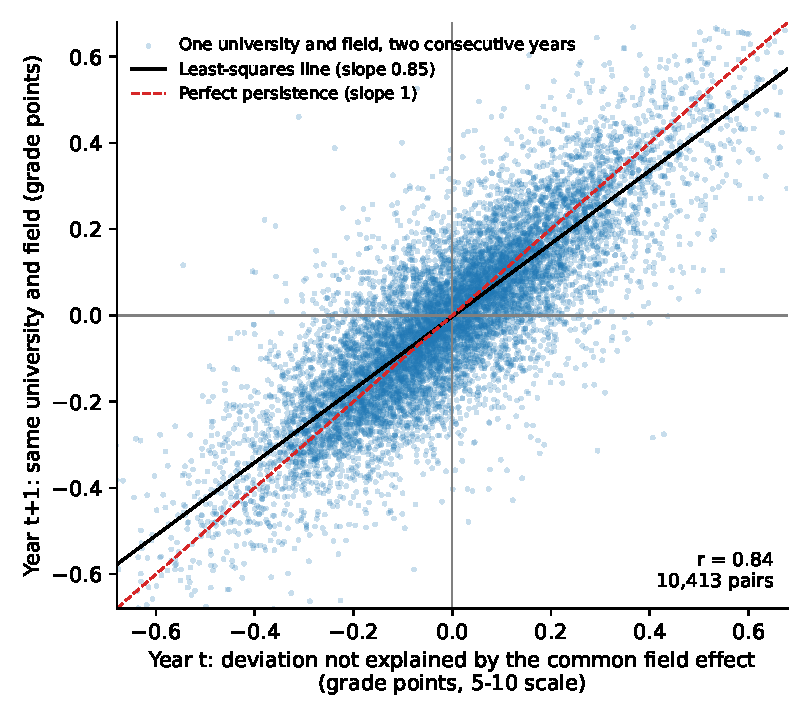
\includegraphics[width=0.5\linewidth]{figures/persistence.pdf}
  \caption{A university's field-specific deviation in one year is close to its deviation the next year. Each blue point is one university and field in two consecutive years. Both axes show the field's distance from its university-year average after subtracting the distance that field has in all universities (grade points, 5--10 scale), in year $t$ and year $t+1$. The black line is the least-squares fit and the dashed red line marks perfect persistence. Data: SIIU, 2015--16 to 2023--24.}
  \label{fig:persistence}
\end{figure}

\begin{figure}[h!]
  \centering
  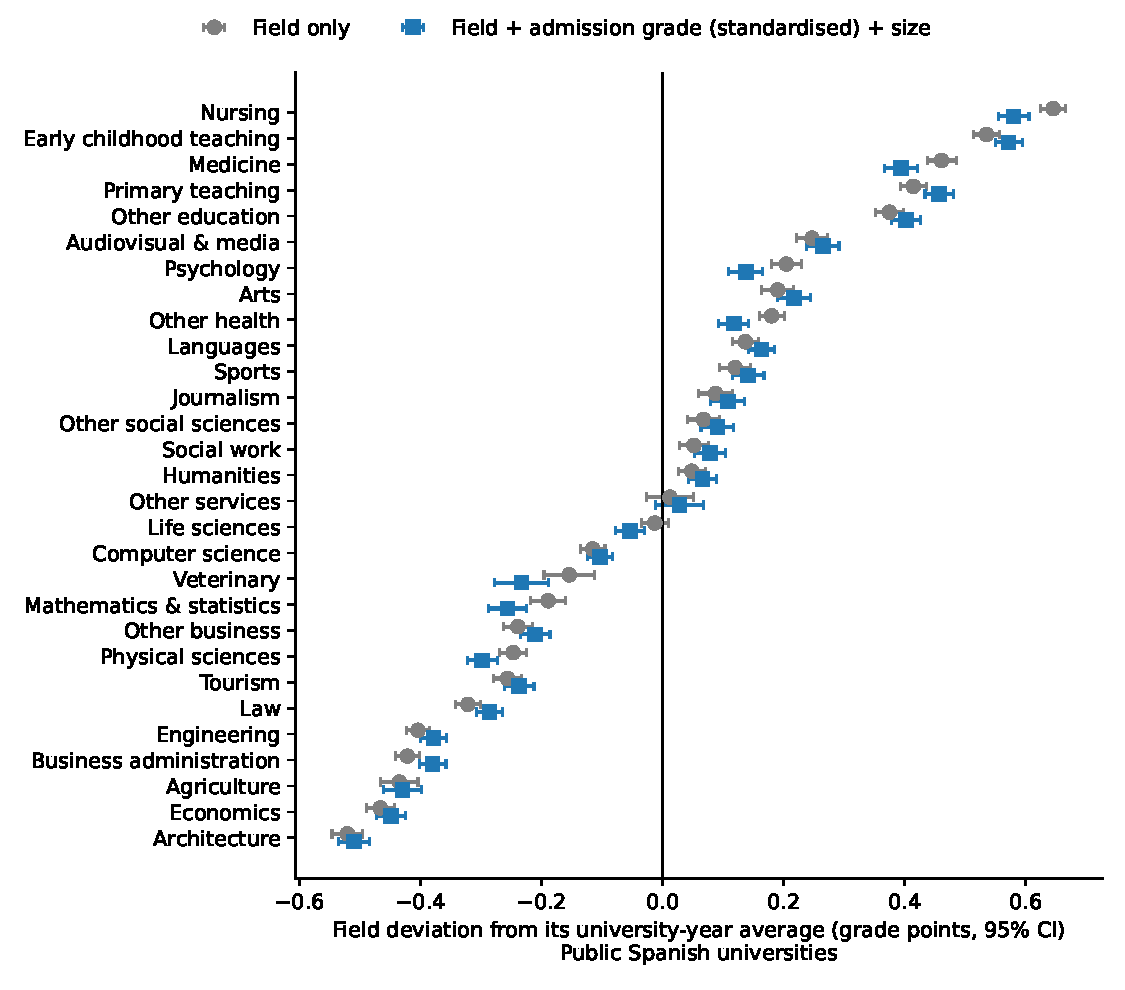
\includegraphics[width=0.62\linewidth]{figures/confounders.pdf}
  \caption{Field effects stay almost the same after controlling for intake and size. Each row shows a field's distance from its university-year average (grade points, 5--10 scale) with a 95\% confidence interval. Grey circles come from a model with the field only; blue squares add the standardised admission grade of the field's branch and the log number of graduates. Positive values mean grades above the university average. 8,042 observations from 47 public universities. Data: SIIU.}
  \label{fig:confounders}
\end{figure}

\clearpage
\section*{Works Cited}
\begin{list}{}{\setlength{\leftmargin}{1.5em}\setlength{\itemindent}{-1.5em}\setlength{\itemsep}{0.3em}}
\item Jeong, Hyun, et al. ``The Construction and Analysis of Course Grades Across Public Universities.'' \textit{Proceedings of the 17th International Conference on Educational Data Mining}, 2024, pp. 643--48, \url{https://doi.org/10.5281/zenodo.12729906}.
\item Ministerio de Ciencia, Innovaci\'on y Universidades. ``Egresados por sexo, grupo de edad y \'ambito de estudio.'' \textit{Estad\'istica de Estudiantes Universitarios}, Sistema Integrado de Informaci\'on Universitaria (SIIU), 2025, \url{https://estadisticas.ciencia.gob.es}. Accessed 24 Oct. 2026.
\item ---. ``Media, cuartiles y m\'aximo de la nota del expediente (estudiantes egresados) por \'ambito de estudio y sexo.'' \textit{Sistema Integrado de Informaci\'on Universitaria (SIIU)}, 2025, \url{https://estadisticas.ciencia.gob.es}. Accessed 10 Oct. 2026.
\item ---. ``Nota media y cuartiles de nota de admisi\'on de los estudiantes de nuevo ingreso en Grado por forma de admisi\'on, sexo y rama de ense\~nanza.'' \textit{Estad\'istica de Estudiantes Universitarios}, Sistema Integrado de Informaci\'on Universitaria (SIIU), 2025, \url{https://estadisticas.ciencia.gob.es}. Accessed 24 Oct. 2026.
\item ---. ``Nota media y cuartiles de nota de admisi\'on de los estudiantes de nuevo ingreso en Grado por forma de admisi\'on, sexo y \'ambito de estudio.'' \textit{Estad\'istica de Estudiantes Universitarios}, Sistema Integrado de Informaci\'on Universitaria (SIIU), 2025, \url{https://estadisticas.ciencia.gob.es}. Accessed 24 Oct. 2026.
\item ---. ``Tasas de abandono del estudio (cohortes de nuevo ingreso en el estudio) por \'ambito de estudio y sexo.'' \textit{Sistema Integrado de Informaci\'on Universitaria (SIIU)}, 2025, \url{https://estadisticas.ciencia.gob.es}. Accessed 24 Oct. 2026.
\item Realinho, Valentim, et al. ``Predict Students' Dropout and Academic Success.'' \textit{UCI Machine Learning Repository}, 2021, \url{https://doi.org/10.24432/C5MC89}.
\end{list}

% ============================================================
\section*{Declaration of Contributions and AI Use}

\textbf{Contributions.} The team agreed on the analysis plan after reading the feedback. Ignacio Gimeno found the data, ran and checked the analysis, and prepared and submitted the report; Adam Bajer and Pablo Torres reviewed the results, the figures and the text.

\textbf{Generative AI.} Ignacio Gimeno used Claude (Anthropic, Claude Code desktop application, October 2026) for three purposes. (1) Data search: it located the Ministry tables on dropout, graduates and admission grades; the team checked each table on the Ministry website. (2) Code: it wrote the Python scripts for the variance decomposition, temporal validation, bootstrap intervals, confounder models, clustering, selection simulation and figures (\texttt{src/progress.py}); the team chose the analyses in response to the feedback, ran the scripts and compared every reported number with the output file \texttt{results/progress\_stats.json}. (3) Text: it drafted the text of this report from the team's instructions and revised its wording; the team reviewed it and is responsible for all content.

\end{document}
